\let\negmedspace\undefined
\let\negthickspace\undefined
\documentclass[article]{IEEEtran}
\usepackage[a5paper, margin=10mm, onecolumn]{geometry}
%\usepackage{lmodern} % Ensure lmodern is loaded for pdflatex
\usepackage{tfrupee} % Include tfrupee package

\setlength{\headheight}{1cm} % Set the height of the header box
\setlength{\headsep}{0mm}     % Set the distance between the header box and the top of the text

\usepackage{gvv-book}
\usepackage{gvv}
\usepackage{cite}
\usepackage{amsmath,amssymb,amsfonts,amsthm}
\usepackage{algorithmic}
\usepackage{graphicx}
\usepackage{textcomp}
\usepackage{xcolor}
\usepackage{txfonts}
\usepackage{listings}
\usepackage{enumitem}
\usepackage{mathtools}
\usepackage{gensymb}
\usepackage{comment}
\usepackage[breaklinks=true]{hyperref}
\usepackage{tkz-euclide} 
\usepackage{listings}                                       
\def\inputGnumericTable{}                                 
\usepackage[latin1]{inputenc}                                
\usepackage{color}                                            
\usepackage{array}                                            
\usepackage{longtable}                                       
\usepackage{calc}                                             
\usepackage{multirow}                                         
\usepackage{hhline}                                           
\usepackage{ifthen}                                           
\usepackage{lscape}

\renewcommand{\thefigure}{\theenumi}
\renewcommand{\thetable}{\theenumi}
\setlength{\intextsep}{10pt} % Space between text and floats

\numberwithin{figure}{enumi}
\renewcommand{\thetable}{\theenumi}

% Marks the beginning of the document
\begin{document}
\bibliographystyle{IEEEtran}
\title{NCERT-9.4.6}
\author{EE24BTECH11035 - KOTHAPALLI AKHIL}
{\let\newpage\relax\maketitle}

\noindent\textbf{Question: }  
Find the solution of the differential equation:  
\begin{equation*}
    \frac{dy}{dx} = (1 + x^2)(1 + y^2).
\end{equation*}

\noindent\textbf{Solution:}  
Rewriting the equation:  
\begin{align}
    \frac{dy}{1 + y^2} = (1 + x^2) dx.
\end{align}

\noindent Integrating both sides:  
\begin{align}
    \int \frac{dy}{1 + y^2} = \int (1 + x^2) dx.
\end{align}

\noindent After simplification:  
\begin{align}
    \tan^{-1}(y) = x + \frac{x^3}{3} + k.
\end{align}
where $k$ is the constant of integration(Here, it is assumed as 0).

\vspace{0.5em}

\noindent\textbf{Numerical Approach:}\\1. I used a for loop for finding the $y$ values as the loop proceeds with iterative formula given below. I took some initial value of $x$ and as loop proceeds I assigned it the value as $x+h$. where $h$ is the step size, representing the rate of change. 
\\2. Assigned the values of $y$ for different $x$-values using a for loop. \\ 
\\ \textbf{Using the Method of Finite Differences}\\
The Method of Finite Differences is a numerical technique used to approximate solutions to differential equations. 

We know that:
\begin{align}
   \lim_{h \to 0} \frac{y(x+h) - y(x)}{h} = \frac{dy}{dx} 
\end{align}
For the given differential equation,
\begin{align}
\frac{dy}{dx} = (1+x^2)(1+y^2)    
\end{align}
we approximate:
\begin{align}
\frac{y_{n+1} - y_n}{h} &\approx (1 + x_n^2)(1 + y_n^2)
\end{align}

This implies:
\begin{align}
y_{n+1} &= y_n + h \cdot (1 + x_n^2)(1 + y_n^2) 
\end{align}

Here, $h$ is the step size, $y_n$ is the approximation of $y(x)$ at the $n$-th step, and $x_n$ is the corresponding $x$-value at the $n$-th step.

\noindent The iterative formula for updating $y$-values is:  
\begin{align}
    y_n = y_{n-1} + \left(\frac{dy}{dx}\right) h,
\end{align}
The iterative formula for updating $x$-values is: 
\begin{align}
    x_n=x_{n-1}+h
\end{align} 

\noindent\textbf{Initial Conditions:}  
\begin{itemize}
    \item $x = 0$  
    \item $y = 0$  
    \item $h = 0.0002$  
\end{itemize}

Using Matplotlib, I plotted the computed points and the graph of the exact solution to verify that they approximately match.
\begin{figure}[h!]
	\centering
	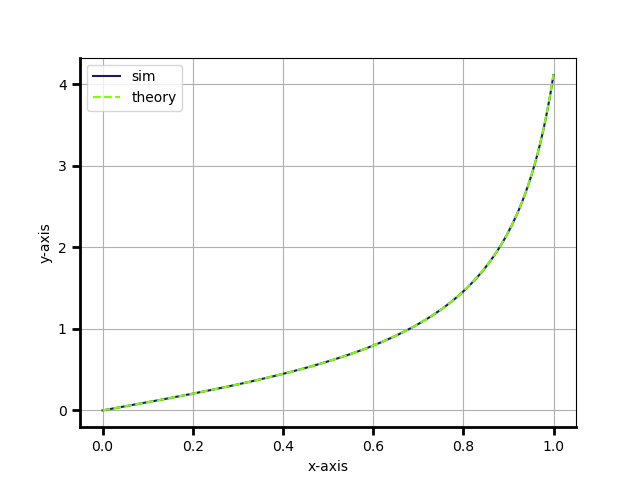
\includegraphics[width=\columnwidth]{figures/Figure_1.png}
	\caption{verifying through graph of sim and theory values}
	\label{stemplot}
\end{figure}	
\end{document}
